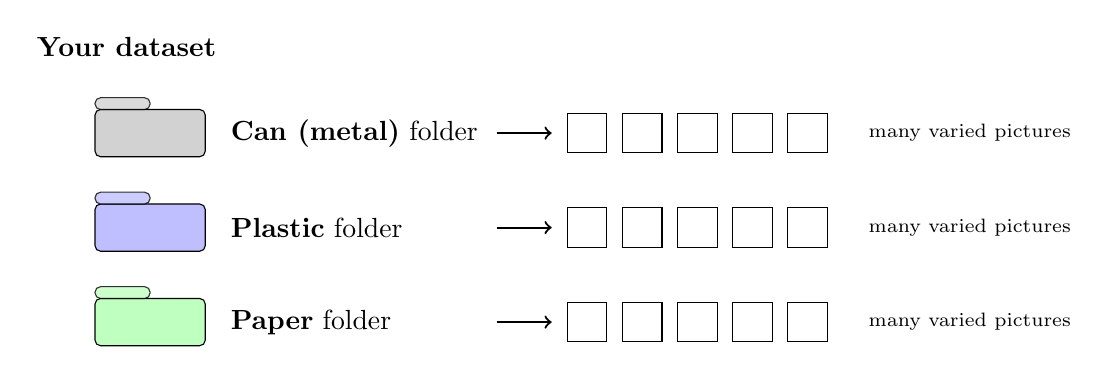
\begin{tikzpicture}[x=1cm,y=1cm]
\node[font=\bfseries] at (0,2.3) {Your dataset};
\foreach \y/\n/\c in {1.2/Can (metal)/gray!35, 0/Plastic/blue!25, -1.2/Paper/green!25}{
 \draw[fill=\c,rounded corners=2pt] (-0.4,\y-0.3) rectangle (1.0,\y+0.3);
 \draw[fill=\c,opacity=0.8,rounded corners=2pt] (-0.4,\y+0.3) rectangle (0.3,\y+0.45);
 \node[anchor=west] at (1.2,\y) {\textbf{\n} folder};
 \foreach \k in {0,1,2,3,4}{\draw[fill=white] (5.6+\k*0.7,\y-0.25) rectangle (6.1+\k*0.7,\y+0.25);}
 \node[anchor=west,font=\scriptsize] at (9.3,\y) {many varied pictures};
}
\draw[thick,->] (4.7,1.2)--(5.4,1.2); \draw[thick,->] (4.7,0)--(5.4,0); \draw[thick,->] (4.7,-1.2)--(5.4,-1.2);
\end{tikzpicture}
